\documentclass[preprint,review,10pt,authoryear,letterpaper]{elsarticle} 
\usepackage[textwidth=5cm]{todonotes} \oddsidemargin -0.5in

\usepackage{graphicx}
\usepackage[subrefformat=parens,labelformat=parens]{subfig}
\usepackage{amsmath,url}
\usepackage{amssymb}
\usepackage{booktabs} % Nicer tables
\usepackage{multirow} % Table cells spanning multiple rows
\usepackage{lineno}
%\usepackage[noperiod]{jabbrv}

\biboptions{comma,sort&compress}

\biboptions{,comma,sort&compress}

\journal{Neuroscience Methods (TBD)}
  
\begin{document}

\begin{frontmatter}

\title{NeuroField: A Neural Field Theory simulation toolbox}


\author{P.K. Fung\corref{ffung}}
\ead{ffung@physics.usyd.edu.au}
\author{R.G. Abeysuriya\corref{}}
\author{X. Zhao\corref{}}

\author{P.A. Robinson\corref{}}

\address{School of Physics, University of Sydney, New South Wales, Australia}
\cortext[ffung]{Corresponding author. Tel. +61 9036 7274}


\begin{abstract}
%% Text of abstract
Neural field models are a powerful, computationally efficient approach to modeling large-scale brain activity. NeuroField is an extensible software package to simulate neural field equations in a wide range of models. The basic element of neural field theory (population activity, wave propagation, and synaptic effects) can be assembled into arbitrary networks and integrated numerically to predict brain activity. NeuroField also includes MATLAB and Python routines for higher-level analysis including the power spectrum. NeuroField is implemented in C++ and has been tested on a range of Linux distributions, Microsoft Windows, and Mac OS X. Extensive user documentation and examples are provided, and typical use of NeuroField does not require C++ experience. NeuroField is open-source and available (http://physics.usyd.edu.au/brain/neurofield) under the GNU license for non-commercial use. 
\end{abstract}

\begin{keyword}
%% keywords here, in the form: keyword \sep keyword
EEG \sep neurophysiology \sep methods \sep modeling
%% MSC codes here, in the form: \MSC code \sep code
%% or \MSC[2008] code \sep code (2000 is the default)

\end{keyword}

\end{frontmatter}

\linenumbers

%% main text
\section{Introduction}
\label{sec:introduction}
Neural field modeling has proved to be a powerful technique for constructing relatively simple, physiologically based models of the brain that are capable of predicting EEG and correlate well with experimental data \cite{Deco2008,Pinotsis2012}. We have developed a neural field corticothalamic model of the brain \citep{Robinson2005,Rowe2004413,PhysRevE.63.021903,PhysRevE.65.041924,Robinson:04aa} that we have previously used to investigate the alpha rhythm \citep{PhysRevE.68.021922,PhysRevE.70.011911}, age-related changes to the physiology of the brain \citep{VanAlbada2010}, evoked response potentials \citep{Rennie2002,ker11}, seizures \citep{Breakspear2006}, and many other phenomena. 

The key features of neural field models are captured by the three key equations governing general neural field theory

\begin{align*}
	D_{ab}V_{ab}(\mathbf{r},t) &= \nu_{ab}\phi_{ab}(\mathbf{r},t),\\
			Q_a(\mathbf{r},t) &= S_a \big[\sum_b V_{ab}(\mathbf{r},t) \big],\\
	\mathcal{D}_{ab}\phi_{ab}(\mathbf{r},t) &= Q_b(\mathbf{r},t-\tau_{ab}).
\end{align*}
which represent synapto-dendritic smoothing, dendritic summation and firing response, and damped wave propagation, respectively. The differential operators are
\begin{align*}
	D_\alpha(t) &= \frac{1}{\alpha\beta}\frac{d^2}{dt^2} + \left( \frac{1}{\alpha} + \frac{1}{\beta}\right) \frac{d}{dt}+1,\\
	\mathcal{D}_a(\mathbf{r},t) &= \frac{1}{\gamma_a^2}\frac{\partial^2}{\partial t^2} + \frac{2}{\gamma_a}\frac{\partial}{\partial t} + 1 - r_a^2\nabla^2,
\end{align*}
and the sigmoid population response $S_a$ is given by
\begin{align*}
	Q_a = S(V_a) = \frac{Q_{\textrm{max}}}{1+\exp[-(V_a - \theta)/\sigma']},
\end{align*}
The relationship between these quantities is schematically illustrated in Fig.~\ref{fig:eirs_cycle}.

\begin{figure}[!b]
\begin{center}
\includegraphics[width=0.40\columnwidth]{EIRS_cycle}
\caption{Schematic overview of the key dynamic quantities of neural field models, and the relationships between them.}
\label{fig:eirs_cycle}
\end{center}
\end{figure}

The most challenging part of applying neural field theory is the implementation of the numerical solver. Several factors contribute to making the numerical integration of neural field equations difficult. In particular, propagation delays between neural populations result in delay-differential equations that require special handling of temporal history. Further, propagation of neural fields according to a damped wave equation adds two dimensions to the system, and requires a relative sophisticated finite-differencing scheme that takes into account the geometry of the system. In addition, periodic boundary conditions must be correctly handled during the integration. 

We have developed NeuroField to provide a software package that solves the neural field equations for arbitrary neural populations, and contains library code for analysis and visualization, thus removing the barriers to quickly testing and analyzing neural field models. The software is designed to be easily extensible with basic C++ programming skills, making it simple to expand upon the basic model to include new phenomena. 

\section{Method and Results}
\label{sec:theory}

\subsection{Key features/Basic functions}
The essential role of NeuroField is to take as input a model and its initial conditions, and to output one or more time series corresponding to the result of integrating the neural field equations. A model is a specification of neural populations (amounting to defining their firing response to input from other populations including synapto-dendritic effects), and connections between the populations including how neural signals propagate through space. Sensory or other stimulus is implemented as a neural population that recieves no input from other populations, and has a pre-defined firing pattern. Integration of the neural field equations provides several quantities of interest. Most notably, the signals from populations can be associated with local field potentials (LFP) or EEG depending, and these predictions can be directly compared against experimental data. The soma potential or firing rate of the neural populations can be compared to individual neuron data. Changes to synaptic strength can be monitored when simulating neural plasticity. When simulating spatially extended populations, spatial correlations and patterns of activity can also be analyzed. 

\missingfigure{Schematic showing blocks for couple, dendrite, qresponse and the relationship between them. Follow the order in which solver evaluates them}

The core of NeuroField is a C++ program that accept a human-readable plain text configuration file. The output from NeuroField is a plain text output file containing all of the requested simulation variables for each time step. The syntax of the output file has been designed to be simple to parse, and the NeuroField package includes reference parsers for Matlab and Python. These parsers may also help serve as a starting point for implementation of parsers other programming languages. 

There are a number of common ways to analyze the output from neural field models. First, plots of the time series are useful for directly viewing neural oscillations, evoked responses, seizures, monitoring plasticiity, and verifying stability. Second, calculation of the power spectrum, which is often compared to experimental EEG. This can also involve detection of multiple spatial modes of activity and incorporation of volume conduction, to account for effects introduced by electrodes in real-world recordings. Finally, spatial patterns of activity and propagation of waves of activity can be visualized on a surface plot. All of these basic analyses are included as Matlab programs in the NeuroField toolbox. 


% \begin{itemize}
% 	\item Specify the parameters for any part of the simulation, including populations, dendritic responses, firing responses, propagators, synapses, stimulus, and output.
% 	% \item Choose alternative wave propagation types, i.e. choose different forms of \(\mathcal{D}_{ab}\);
% 	% \item Uses plastic synapses, i.e. \(\nu_{ab}=\nu_{ab}(\mathbf{r},t)\).
% 	% \item Use different firing responses, i.e. change \(S_a\).
% \end{itemize}

\subsection{Data structures}

NeuroField solves each part of the neural field model with an object:
\begin{align*}
	P &= \nu_{ab}\phi_{ab}, & \mathtt{Couple}\\
	D_{ab}V_{ab} &= P, & \mathtt{Dendrite}\\
	Q_a &= S_a \big[\sum_b V_{ab} \big], & \mathtt{QResponse/Pop}\\
	\mathcal{D}_{ab}\phi_{ab} &= Q_b,&  \mathtt{Propag}
\end{align*}
The behavior of each of these objects encapsulates the details of the neural field equations.

\subsubsection{Populations}
A population contains a QResponse object, which defines how the population potential is mapped to firing rate. The QResponse may return the sigmoid of the voltage, as written above. Alternatively it could be an arbitrary function, such as a linearized version of the sigmoid. Effects like bursting can also be included.

\todo[inline]{Code snippets}

\subsubsection{Propagators}
The neural field generated by a population propagates according to the associated Propagator. For populations where spatial propagation effects are insignificant, this propagator may simply be unity. The propagator object takes into account the spatial geometry of the problem, so can be applied to both 2D sheets and spherical geometries. 

\todo[inline]{Code snippets}

\subsubsection{Couples}
The coupling strength of a connection is typically constant, but can be an arbitrary function of a range of different factors, allowing modeling of a wide variety of plasticity effects including STDP and CaDP

\subsubsection{Input and output}

\begin{itemize}
	\item  Mention structure of config and output files
	\item Largely human readable, but relatively simple to construct and parse programatically
	\item Examples of the output file
\end{itemize}

\todo[inline]{Example output, few times, maybe 2 nodes 2 traces}

\subsection{Visualization and analysis}

\subsubsection{Helper scripts}
NeuroField is packaged with several helper scripts written in MATLAB to assist with running, analyzing and visualizing models. 

\subsubsection{Reading output files}
nf\_read() allows users to parse the output file from NeuroField into a MATLAB struct object.
nf\_grid reshapes the output for handling matrices. 

\subsubsection{Writing config files}
nf\_eirs() demonstrates writing a configuration file, running it with nf\_run(), and then reading it with nf\_read(). This demonstrates a complete MATLAB-based toolchain for using NeuroField.

\subsubsection{Calculating power spectra}
The power spectrum can be obtained by FFT, but correct normalization and calculation of the power spectrum including multiple spatial modes can be challenging to implement. We have implemented a 3D FFT algorithm that correctly normalizes the output and includes volume conduction effects that selective attenuate spatial modes depending on their wavenumber. The result can be directly compared to analytical predictions.

\begin{figure}[!b]
\begin{center}
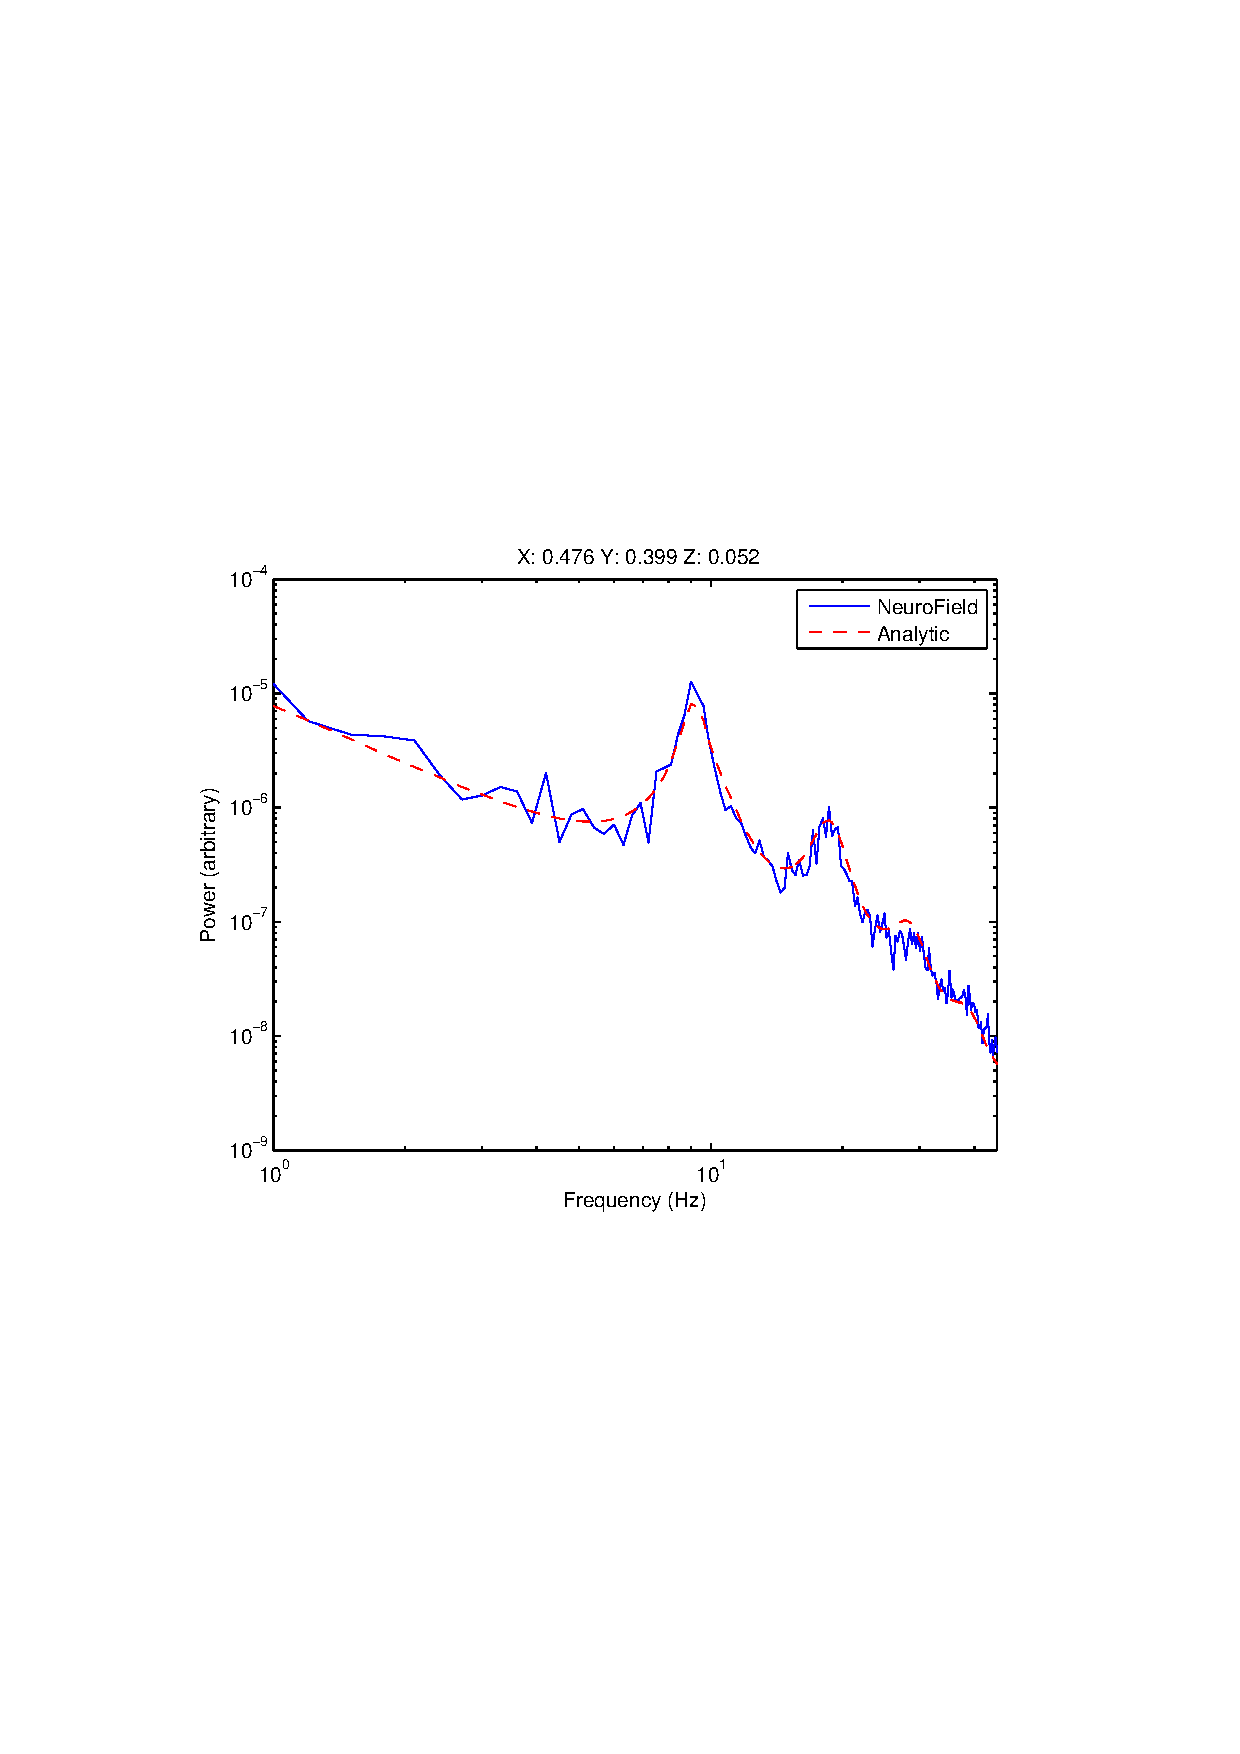
\includegraphics[width=0.80\columnwidth]{corticothalamic_comparison}
\caption{Comparision of linear analytic spectrum with the power spectrum computed using the NeuroField package analysis tools.}
\label{fig:ct_spectrum}
\end{center}
\end{figure}

\subsubsection{Visualizing output}
The nf\_extract() function makes it easy to select data for plotting from a NeuroField object.  
nf\_movie can plot an animation of the output


% \section{Results}

% In this section, we present examples of NeuroField applied to recent research.

% \subsection{Corticothalamic model (Romesh)}

% \begin{figure}[!b]
% \begin{center}
% \includegraphics[width=0.40\columnwidth]{EIRS_clean}
% \caption{Wake EC, same params as already published}
% \label{fig:ct_schematic}
% \end{center}
% \end{figure}


% \begin{figure}[!b]
% \begin{center}
% 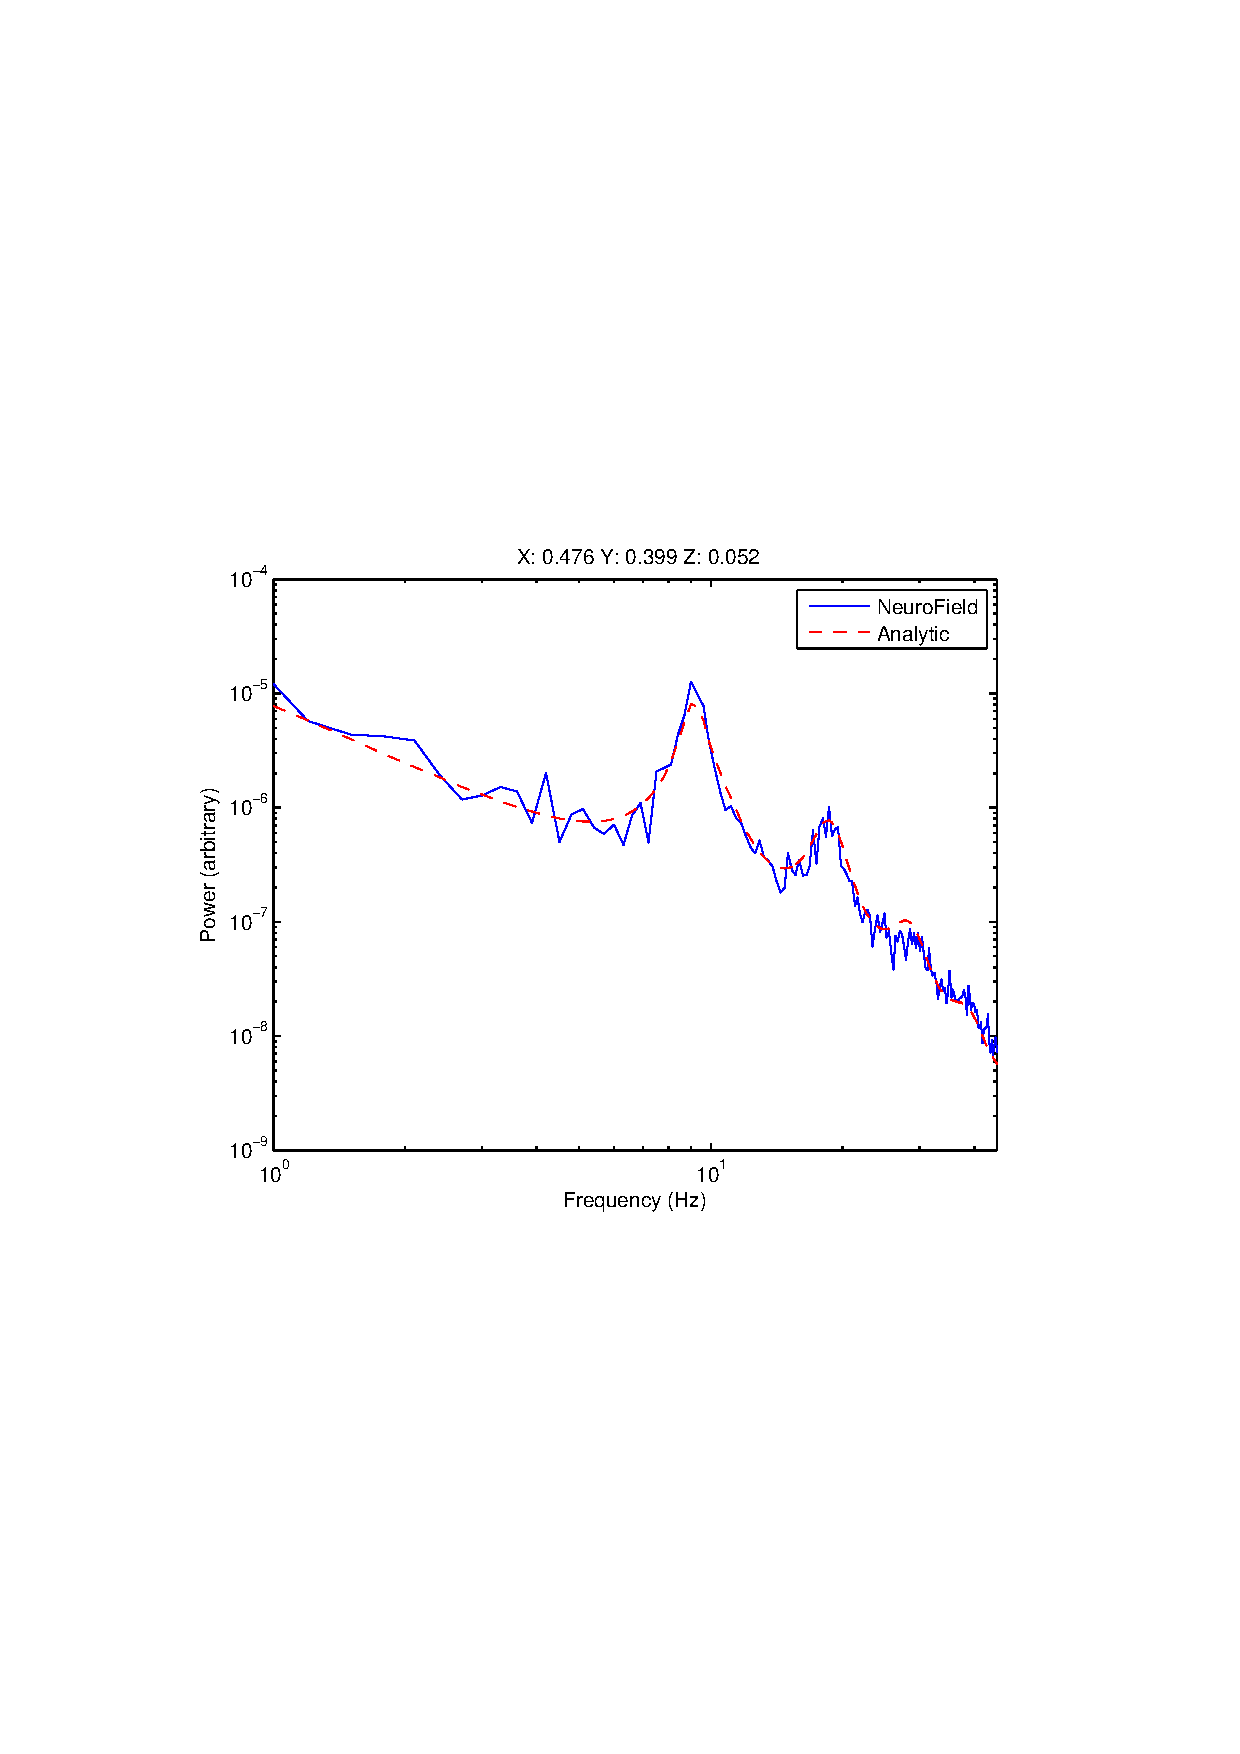
\includegraphics[width=0.40\columnwidth]{corticothalamic_comparison}
% \caption{Wake EC, same params as already published}
% \label{fig:ct_spectrum}
% \end{center}
% \end{figure}


% \begin{itemize}
% 	\item Sleep spindles
% 	\item Wake alpha peak
% 	\item Volume conduction
% \end{itemize}

% \subsection{Plasticity (Felix)}

% \subsection{Bursting (XL)}

% \subsection{Seizures (XL, Romesh)}

\section{Discussion}
\label{sec:discussion}

We have developed NeuroField to provide an extensible, reliable framework for integrating nonlinear delay differential equations including spatial propagation. NeuroField is aimed for use by researchers who have constructed neural field models of the brain that require numerical integration. In this section, we review some usage and performance considerations.

\subsection{White noise stimulus}
\begin{itemize}
	\item White noise requires stocastic DE integrator, effectively Euler
	\item Noise amplitude depends on grid resolution as this affects the possible bandwidth. Similar features depend on frequency domain power so noise needs to be normalized correctly
\end{itemize}

\subsection{Performance}

\begin{itemize}
\item Some numbers about the runtime and memory requirements of NeuroField
\item Note that the memory requirements scale with the grid size, and the grid size depends on Lx and the propagator lengths (automatically enforced)
\item Also that the delays in the system cause O(n) increases in memory usage
\end{itemize}


\section{Acknowledgements}
\label{sec:acknowledgements}
This work was supported by the Australian Research Council, National Health and Medical Research Council (through the Center for Integrated Research and Understanding of Sleep), and the Westmead Millennium Institute.

\section{References}
\bibliographystyle{elsarticle-harv}
\bibliography{neurofield}

\end{document}

%% References
%%
%% Following citation commands can be used in the body text:
%%
%%  \citet{key}  ==>>  Jones et al. (1990)
%%  \citep{key}  ==>>  (Jones et al., 1990)
%%
%% Multiple citations as normal:
%% \citep{key1,key2}         ==>> (Jones et al., 1990; Smith, 1989)
%%                            or  (Jones et al., 1990, 1991)
%%                            or  (Jones et al., 1990a,b)
%% \citep{key} is the equivalent of \citet{key} in author-year mode
%%
%% Full author lists may be forced with \citet* or \citep*, e.g.
%%   \citep*{key}            ==>> (Jones, Baker, and Williams, 1990)
%%
%% Optional notes as:
%%   \citep[chap. 2]{key}    ==>> (Jones et al., 1990, chap. 2)
%%   \citep[e.g.,][]{key}    ==>> (e.g., Jones et al., 1990)
%%   \citep[see][pg. 34]{key}==>> (see Jones et al., 1990, pg. 34)
%%  (Note: in standard LaTeX, only one note is allowed, after the ref.
%%   Here, one note is like the standard, two make pre- and post-notes.)
%%
%%   \citealt{key}          ==>> Jones et al. 1990
%%   \citealt*{key}         ==>> Jones, Baker, and Williams 1990
%%   \citealp{key}          ==>> Jones et al., 1990
%%   \citealp*{key}         ==>> Jones, Baker, and Williams, 1990
%%
%% Additional citation possibilities
%%   \citeauthor{key}       ==>> Jones et al.
%%   \citeauthor*{key}      ==>> Jones, Baker, and Williams
%%   \citeyear{key}         ==>> 1990
%%   \citeyearpar{key}      ==>> (1990)
%%   \citetext{priv. comm.} ==>> (priv. comm.)
%%   \citenum{key}          ==>> 11 [non-superscripted]
%% Note: full author lists depends on whether the bib style supports them;
%%       if not, the abbreviated list is printed even when full requested.
%%
%% For names like della Robbia at the start of a sentence, use
%%   \Citet{dRob98}         ==>> Della Robbia (1998)
%%   \Citep{dRob98}         ==>> (Della Robbia, 1998)
%%   \Citeauthor{dRob98}    ==>> Della Robbia


%% References with bibTeX database:

%% Authors are advised to submit their bibtex database files. They are
%% requested to list a bibtex style file in the manuscript if they do
%% not want to use elsarticle-harv.bst.

%% References without bibTeX database:

% \begin{thebibliography}{00}

%% \bibitem must have one of the following forms:
%%   \bibitem[Jones et al.(1990)]{key}...
%%   \bibitem[Jones et al.(1990)Jones, Baker, and Williams]{key}...
%%   \bibitem[Jones et al., 1990]{key}...
%%   \bibitem[\protect\citeauthoryear{Jones, Baker, and Williams}{Jones
%%       et al.}{1990}]{key}...
%%   \bibitem[\protect\citeauthoryear{Jones et al.}{1990}]{key}...
%%   \bibitem[\protect\astroncite{Jones et al.}{1990}]{key}...
%%   \bibitem[\protect\citename{Jones et al., }1990]{key}...
%%   \harvarditem[Jones et al.]{Jones, Baker, and Williams}{1990}{key}...
%%

% \bibitem[ ()]{}

% \end{thebibliography}

%%
%% End of file `elsarticle-template-harv.tex'.
